\documentclass{article}
\usepackage[utf8]{inputenc}
\usepackage{subfig}

%References
\usepackage{natbib}
%IMPORTANT use https://www.citationmachine.net/ if you need to generate references!
% \citep{reference} creates Harvard Style references throughout

%Colors
\usepackage{xcolor}

\usepackage[protrusion=true,expansion]{microtype}

%Code Markup
\usepackage[outputdir=cache]{minted}
%Syntax Highlighting Style
\definecolor{bggray}{RGB}{40,40,40}
%Macro to make a Syntax Highlighter For Java files 
%Use \javacode{filename.java} to insert a Java File W/ Syntax Highlighting file into the PDF
\newmintedfile[javacode]{java}{
	style=fruity,
	bgcolor=bggray,
	linenos,
	breaklines,
	tabsize=2,
	obeytabs
}

\newmintedfile[bashoutput]{txt}{
	style=fruity,
	bgcolor=lightgray,
	breaklines,
	tabsize=2,
	obeytabs
}

\newmintedfile[ccode]{c}{
	style=fruity,
	bgcolor=bggray,
	linenos,
	breaklines,
	tabsize=2,
	obeytabs
}

%Page Margins and stuff
\usepackage{geometry}
 \geometry{
 a4paper,
 total={170mm,257mm},
 left=20mm,
 }

%Pictures
\usepackage{graphicx}
\graphicspath{ {./images/} }

%Move the title position
\usepackage{titling}

\setlength{\droptitle}{-8.5em} %Up, near the top but not too high

\title{Assignment 1 - Programming Paragdims}
\author{Daniel Hannon (19484286)}
\date{October 2021}

\begin{document}
	\maketitle
	\section{Question 1}
		\subsection{Code}
			\ccode{assignment.c}
		\subsection{Output}
			\begin{figure}[h!]
				\centering
				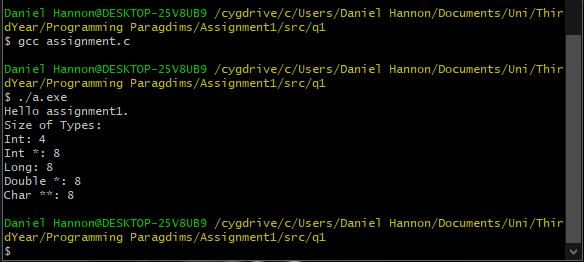
\includegraphics[width=0.7\textwidth]{1.png}
			\end{figure}
		\subsection{Comments}
			\begin{enumerate}
				\item Int has size 4 as it is 4 bytes(32 bits long)
				\item Long has size 8 as it is 8 bytes long (64 bytes)
				\item All the pointers (Int *, Double *, Char **) have length 8 as I am using a 64bit operating system and thus all pointers reference a 64 bit address. If I were using a 32 bit operating system, the pointers would be 32 bits long
			\end{enumerate}
	\section{Question 2}
		\subsection{Code}
			\subsubsection{Code I wrote for linkedlist.h}
				\ccode{assignment2.c}
				\newpage
			\subsubsection{tests.c}
				\ccode{tests2.c}
		\newpage
		\subsection{Output}
			\begin{figure}[h!]
				\centering
				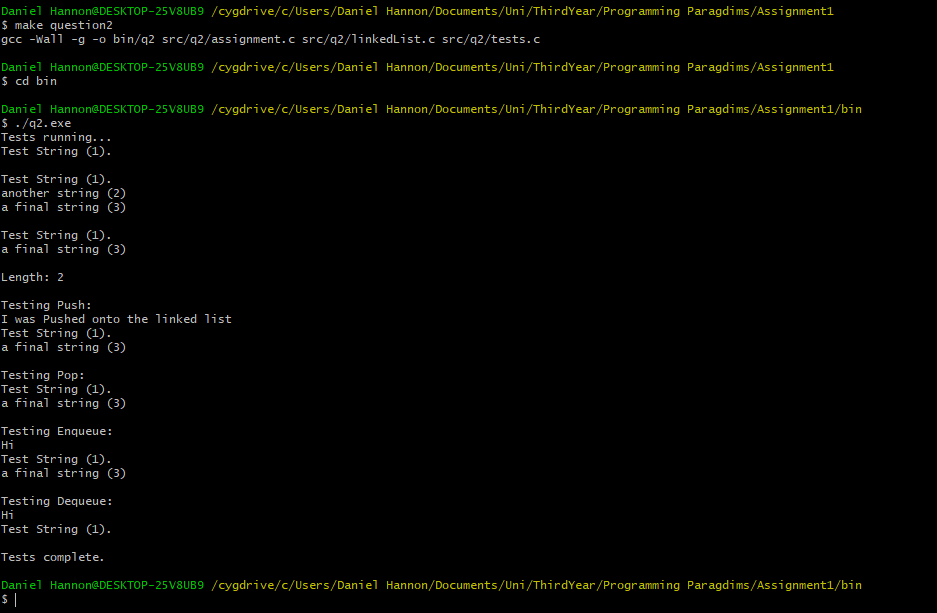
\includegraphics[width=0.7\textwidth]{2.png}
			\end{figure}
	\section{Question 3}
		\subsection{Code}
			\subsubsection{assignment.c}
				\ccode{assignment3.c}
			\subsubsection{genericLinkedList.c}
				\ccode{genericLinkedList.c}
			\subsubsection{tests.c}
				\ccode{tests3.c}
		\newpage
		\subsection{Output}
			\begin{figure}[h!]
				\centering
				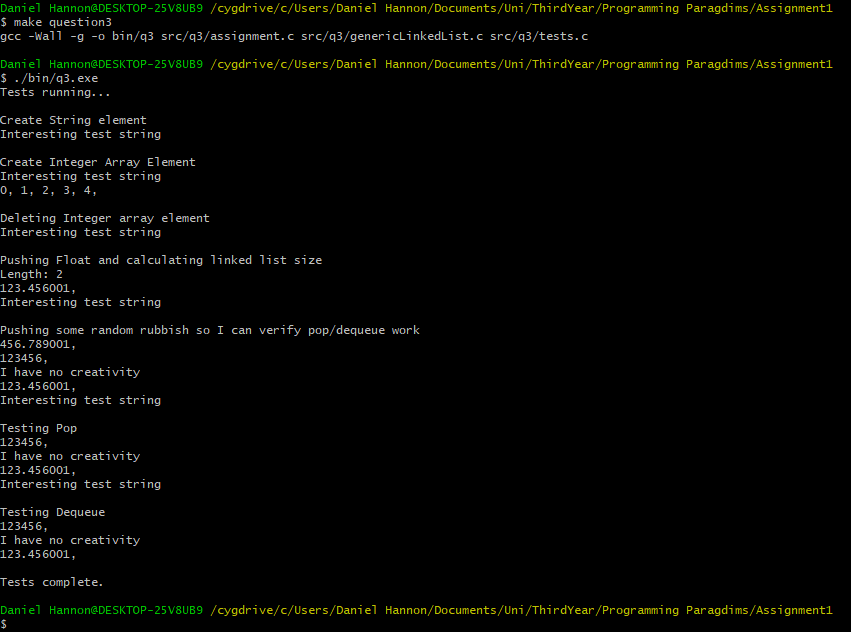
\includegraphics[width=0.7\textwidth]{3.png}
			\end{figure}
		\subsection{Comments}
			In Order to achieve the generic linkedlist I had to figure out how to pass a function as an arguement and stuff, I wrote the print functions in a way that would ensure that I could print arrays as I felt that would be cool and practical.\\fptr is defined as "typedef void(*fptr)(void *,size\_t);" in genericLinkedList.h\\When it came to copying the data for the pointers I used memcpy as it seemed to be the logical solution
	\section{Question 4}
		\subsection{Reversing a Singly Linked List}
			What seems to  be the logical way to traverse a singly linked list is to create a stack and push every element to the stack and then at the end you can traverse that as it is the linked list in a reversed order, Albeit it requires you to make a copy of the linked list and thus it will occupy a total of twice the total memory occuppied by the Linked List.  It would also require you to recreate the stack every time that the linked list is updated which could become quite computationally expensive as the linked list becomes larger.
		\subsection{Possible method to make it less expensive in terms of memory and computation}
			A way to deal with this would be to instead of having a Singly-Linked List we could make it a Doubly-Linked List, that being each element has a pointer to the element before it in the linked list. instead of occupying twice the memory for a reverse traversal, it would occupy 4/8 bytes extra per node depending on whether or not you have a 32 or 64 bit operating system. In order to get the reverse of the linked list we would require to search to the end and then simply use the pointer to the previous node on each node until you return to the start. In order to eliminate that we could make the list circular (Last node has the first one as the next one and vice versa) but that might require extra memory as you would need some way to determine if you reached the start again 
	%Sets to Harvard Style and links the references file
	\bibliographystyle{agsm}
	\bibliography{references}
\end{document}